\documentclass[journal]{IEEEtran}
\usepackage[a5paper, margin=10mm, onecolumn]{geometry}
\usepackage{lmodern}
\usepackage{tfrupee}
\setlength{\headheight}{1cm}
\setlength{\headsep}{0mm}

\usepackage{gvv-book}
\usepackage{gvv}
\usepackage{cite}
\usepackage{amsmath,amssymb,amsfonts,amsthm}
\usepackage{algorithmic}
\usepackage{graphicx}
\usepackage{textcomp}
\usepackage{xcolor}
\usepackage{txfonts}
\usepackage{listings}
\usepackage{enumitem}
\usepackage{mathtools}
\usepackage{gensymb}
\usepackage{comment}
\usepackage[breaklinks=true]{hyperref}
\usepackage{tkz-euclide}
\usepackage{listings}
\def\inputGnumericTable{}
\usepackage[latin1]{inputenc}
\usepackage{color}
\usepackage{array}
\usepackage{longtable}
\usepackage{calc}
\usepackage{multirow}
\usepackage{hhline}
\usepackage{ifthen}
\usepackage{lscape}
\usepackage{xparse}

\bibliographystyle{IEEEtran}

\title{2.10.71}
\author{EE25BTECH11043 - Nishid Khandagre} % Replace with your name

\begin{document}
\maketitle

\renewcommand{\thefigure}{\theenumi}
\renewcommand{\thetable}{\theenumi}

\numberwithin{equation}{enumi}
\numberwithin{figure}{enumi}

\textbf{Question}:\
If the vectors $\vec{b}$, $\vec{c}$, $\vec{d}$ are not coplanar, then prove that the vector
$\myvec{\vec{a} \times\vec{b}} \times\myvec{\vec{c} \times\vec{d}} + \myvec{\vec{a} \times\vec{c}} \times\myvec{\vec{d} \times\vec{b}} + \myvec{\vec{a} \times\vec{d}} \times\myvec{\vec{b} \times\vec{c}}$
is parallel to $\vec{a}$.

\textbf{Solution: }

The vector triple product $\vec{A} \times \myvec{\vec{B} \times \vec{C}}$ can be written as:
\begin{align}
\vec{A} \times \myvec{\vec{B} \times \vec{C}} &= \vec{B}\myvec{\vec{A}^\top \vec{C}} - \vec{C}\myvec{\vec{A}^\top \vec{B}}
\end{align}
Also, we know

\begin{align}
\myvec{\vec{A} \times \vec{B}} \times \vec{C} = - \vec{C} \times \myvec{\vec{A} \times \vec{B}}
\end{align}


\begin{align}
\myvec{\vec{A} \times \vec{B}} \times \myvec{\vec{C} \times \vec{D}} = \myvec{\vec{A}^\top \myvec{\vec{C} \times \vec{D}}} \vec{B} - \myvec{\vec{B}^\top \myvec{\vec{C} \times \vec{D}}} \vec{A}
\label{eq:equation}
\end{align}


by using \eqref{eq:equation}
\begin{align}
\myvec{\vec{a} \times\vec{b}}\times \myvec{\vec{c} \times\vec{d}}&= \myvec{\vec{a}^\top \myvec{\vec{c} \times \vec{d}}} \vec{b} - \myvec{\vec{b}^\top \myvec{\vec{c} \times \vec{d}}} \vec{a}\\
&=\sbrak{\vec{a} \ \vec{c} \ \vec{d}}\vec{b} - \sbrak{\vec{b} \ \vec{c} \ \vec{d}}\vec{a}
\end{align}

\begin{align}
\myvec{\vec{a} \times\vec{c}} \times\myvec{\vec{d} \times\vec{b}}&=
\myvec{\vec{a}^\top \myvec{\vec{d} \times \vec{b}}} \vec{c} - \myvec{\vec{c}^\top \myvec{\vec{d} \times \vec{b}}} \vec{a}\\
&= \sbrak{\vec{a} \ \vec{d} \ \vec{b}}\vec{c} - \sbrak{\vec{c} \ \vec{d} \ \vec{b}}\vec{a} \\
&= -\sbrak{\vec{a} \ \vec{b} \ \vec{d}}\vec{c} + \sbrak{\vec{b} \ \vec{c} \ \vec{d}}\vec{a}
\end{align}

\begin{align}
\myvec{\vec{a} \times\vec{d}} \times\myvec{\vec{b} \times\vec{c}}&=
\myvec{\vec{a}^\top \myvec{\vec{b} \times \vec{c}}} \vec{d} - \myvec{\vec{d}^\top \myvec{\vec{b} \times \vec{c}}} \vec{a}\\
&=\sbrak{\vec{a} \ \vec{b} \ \vec{c}}\vec{d} - \sbrak{\vec{d} \ \vec{b} \ \vec{c}}\vec{a}  \\
&= \sbrak{\vec{a} \ \vec{b} \ \vec{c}}\vec{d} - \sbrak{\vec{b} \ \vec{c} \ \vec{d}}\vec{a}
\end{align}

Adding equations (1), (2), and (3):
\begin{align}
\myvec{\vec{a} \times\vec{b}} \times\myvec{\vec{c} \times\vec{d}} + \myvec{\vec{a} \times\vec{c}} \times\myvec{\vec{d} \times\vec{b}} + \myvec{\vec{a} \times\vec{d}} \times\myvec{\vec{b} \times\vec{c}}\\
\end{align}
\begin{align}
&= \sbrak{\vec{a} \ \vec{c} \ \vec{d}}\vec{b} - \sbrak{\vec{b} \ \vec{c} \ \vec{d}}\vec{a}-\sbrak{\vec{a} \ \vec{b} \ \vec{d}}\vec{c} + \sbrak{\vec{b} \ \vec{c} \ \vec{d}}\vec{a}+\sbrak{\vec{a} \ \vec{b} \ \vec{c}}\vec{d} - \sbrak{\vec{b} \ \vec{c} \ \vec{d}}\vec{a}\\
&= \sbrak{\vec{a} \ \vec{c} \ \vec{d}}\vec{b} - \sbrak{\vec{a} \ \vec{b} \ \vec{d}}\vec{c} + \sbrak{\vec{a} \ \vec{b} \ \vec{c}}\vec{d} - \sbrak{\vec{b} \ \vec{c} \ \vec{d}}\vec{a}
\end{align}
Using the expansion of a vector $\vec{a}$ in terms of non-coplanar vectors $\vec{b}, \vec{c}, \vec{d}$:
\begin{align}
\vec{a}\sbrak{\vec{b} \ \vec{c} \ \vec{d}} = \sbrak{\vec{a} \ \vec{c} \ \vec{d}}\vec{b} + \sbrak{\vec{a} \ \vec{d} \ \vec{b}}\vec{c} + \sbrak{\vec{a} \ \vec{b} \ \vec{c}}\vec{d}
\end{align}
Rearranging the scalar triple products on the right:
\begin{align}
\vec{a}\sbrak{\vec{b} \ \vec{c} \ \vec{d}} = \sbrak{\vec{a} \ \vec{c} \ \vec{d}}\vec{b} - \sbrak{\vec{a} \ \vec{b} \ \vec{d}}\vec{c} + \sbrak{\vec{a} \ \vec{b} \ \vec{c}}\vec{d}
\end{align}
Substitute this into the sum:
\begin{align}
&= \vec{a}\sbrak{\vec{b} \ \vec{c} \ \vec{d}} - \sbrak{\vec{b} \ \vec{c} \ \vec{d}}\vec{a} \\
&= \sbrak{\vec{b} \ \vec{c} \ \vec{d}}\vec{a} - \sbrak{\vec{b} \ \vec{c} \ \vec{d}}\vec{a} \\
&= \vec{0}
\end{align}
The resultant vector is $\vec{0}$.\\ A zero vector is considered parallel to any vector.
Thus, the given vector expression is parallel to $\vec{a}$.



\begin{figure}[H]
   \centering
  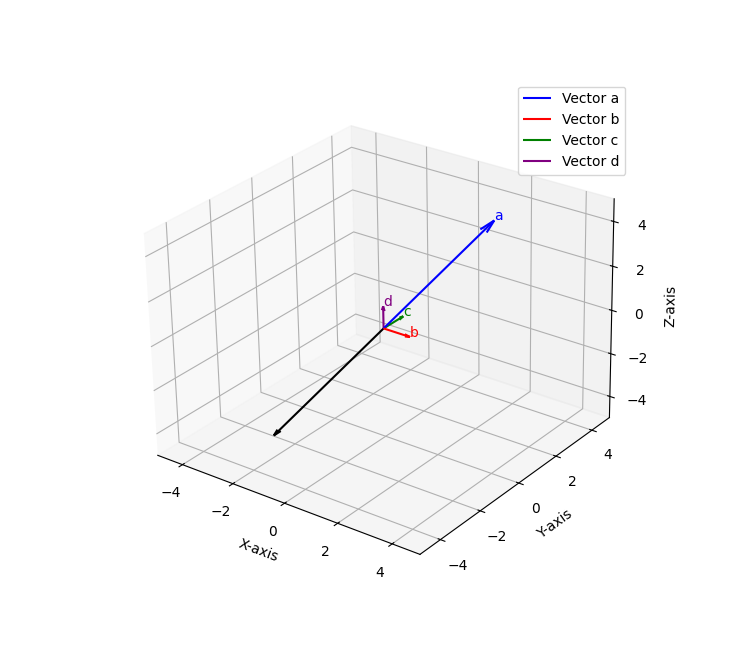
\includegraphics[width=0.7\columnwidth]{figs/fig1.png}
   \caption{}
   \label{fig:1}
\end{figure}


\end{document}
